\documentclass[14pt]{beamer}

\usepackage{listings}
\lstloadlanguages{python}

\usepackage{color}
\usepackage{tikz}


\mode<presentation>
{
\usetheme{AlpesLasers}
\setbeamercovered{transparent}
  %\setbeamertemplate{footline}[frame number] 
  %\setbeamertemplate{navigation symbols}{ 
  %\hskip 0.3cm
  %\insertframenumber / \inserttotalframenumber  % <<< frame #
  %\insertpagenumber / \insertpresentationendpage % <<< page #
%} 
}

% font definitions, try \usepackage{ae} instead of the following
% three lines if you don't like this look
\usepackage{mathptmx}
\usepackage[scaled=.90]{helvet}
\usepackage{courier}
\usepackage[T1]{fontenc}
\usepackage[english]{babel}
\usepackage[latin1]{inputenc}
\title{Infrared receptors in pyrophilous\\ ("fire loving") insects as model for new un-cooled infrared sensors (2011)}
\subtitle{A Golay Cell overview}
\author{St\'ephane Poss}
\date{June 30th 2014}
% This is only inserted into the PDF information catalog. Can be left
% out.
\subject{ALDIRAC}


\begin{document}
\begin{frame}[plain]
\titlepage
\end{frame}

\section{Introduction}

\begin{frame}
\tableofcontents
\end{frame}

\section{The authors}
\begin{frame}
\frametitle{The authors}
\begin{enumerate}
\item David Klocke
\item Anke Schmitz
\item Helmut Soltner
\item Herbert Bousack
\item Helmut Schmitz*
\end{enumerate}
Institute of zoology, University of Bonn,\\
Forschungszentrum Julich GmbH, Zentralabteilung Technologie,\\
Forschungszentrum Julich GmbH, Perter Grunberg Institut
\end{frame}

\section{A bit of biology}
\begin{frame}
\frametitle{Fire loving beetles?}
\begin{quote}
Fire loving (pyrophilous) insects depend on forest fires for their reproduction.
\end{quote}
\begin{columns}
\column{0.49\textwidth}
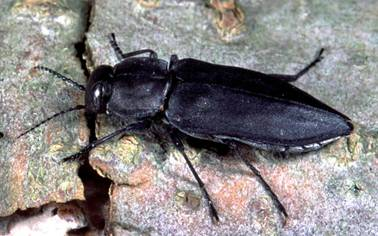
\includegraphics[width=\textwidth]{kaefer_03.jpg}
\column{0.49\textwidth}
\begin{quote}
[...] these insects have special sensors for smoke and infrared radiation.
\end{quote}
\end{columns}
\end{frame}

\begin{frame}
\frametitle{How/why}
\begin{itemize}
\item Often stay on the stem of trees close to burning or glowing wood or hot ashes
\item They try to copulate vigorously
\item Females deposit the eggs under the bark of burnt trees
\item The larvae can \emph{only} develop in the wood of burnt trees
\end{itemize}
Fire detection is obviously an important requirement for the survival of the pyrophilous insects
\end{frame}

\begin{frame}
\frametitle{Requirements/solution}
\begin{itemize}
\item Must be able to detect heat from a distances as large as possible
\item Ability to avoid ``hot'' spots $>60^oC$ (dangerous)
\end{itemize}
Solution:\\
\begin{quote}
\alert{These insects feature so-called photomechanic IR receptors} which might serve well as models for the technical design of un-cooled IR receptors.
\end{quote}
\end{frame}

\begin{frame}
\frametitle{Mechanoreceptors}
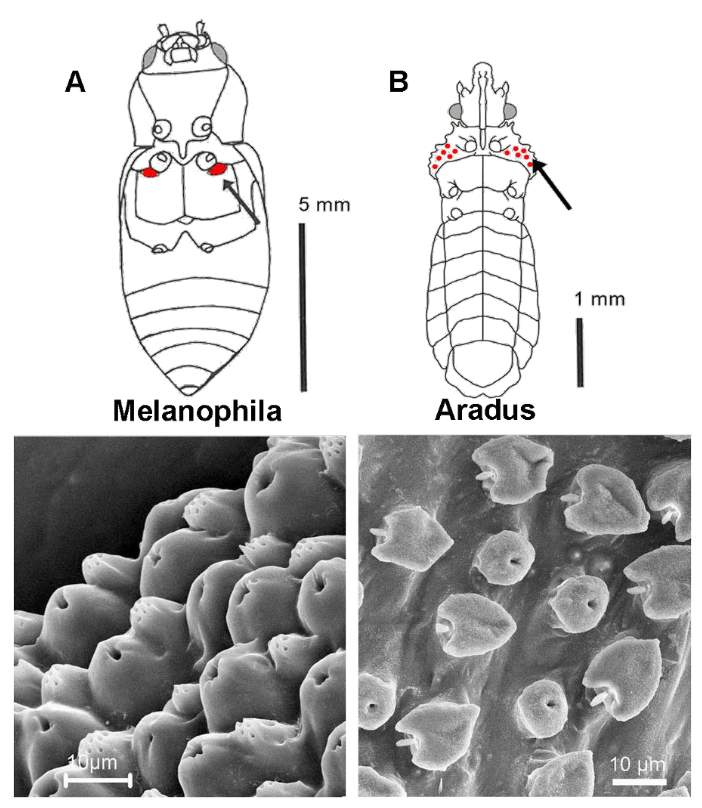
\includegraphics[width=7cm]{beetles_sensors.png}
\end{frame}
\begin{frame}
\frametitle{Mechanoreceptors}
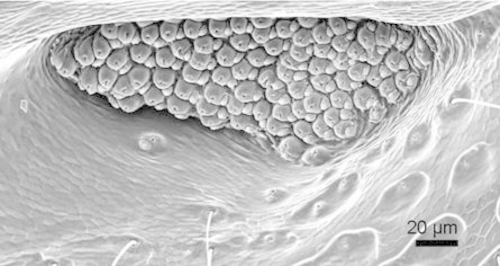
\includegraphics[width=8cm]{6974e8e62f.jpg}\\
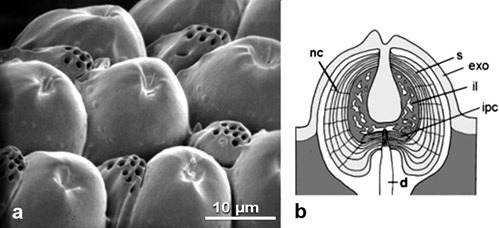
\includegraphics[width=8cm]{IR_sensor_abb_3_02.jpg}
\end{frame}
\begin{frame}
\frametitle{Mechanoreceptors}
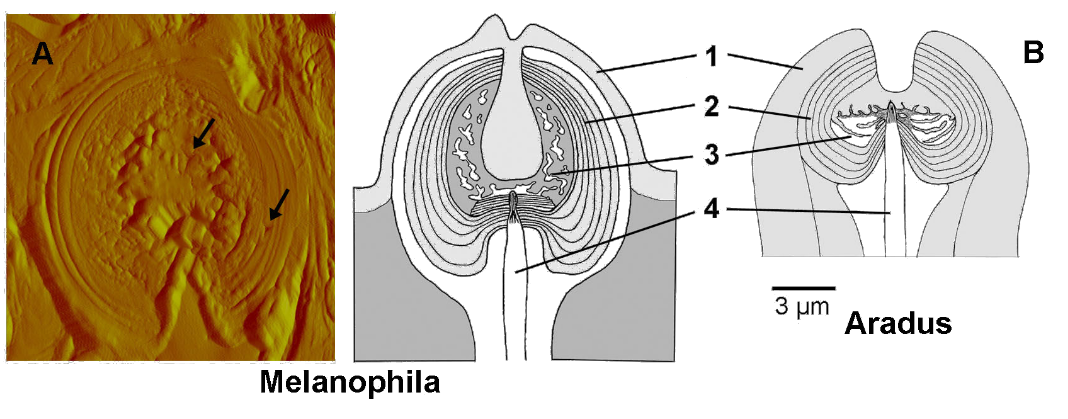
\includegraphics[width=10cm]{mechanoreceptor.png}
\begin{enumerate}
\item outer exocuticle (hard)
\item exocuticular shell of the inner sphere (hard)
\item microfluidic core
\item tip of the mechanosensory dendrite
\end{enumerate}
\end{frame}


\begin{frame}
\frametitle{Working principles}
\begin{quote}
Most probably, IR radiation absorbed by the proteins, the chitin fibres, and the water of the sensillum heats up the sphere, which immediately causes \alert{thermal expansion} especially of the liquid inside the microfluidic core.
\end{quote}
\begin{quote}
[...] the only \alert{compliant structure} in the sphere is the \alert{membrane} of the tip of the \alert{mechanosensitive dendrite.}
\end{quote}
\end{frame}

\section{Golay cell}
\begin{frame}
\frametitle{A look into the Golay Cell}
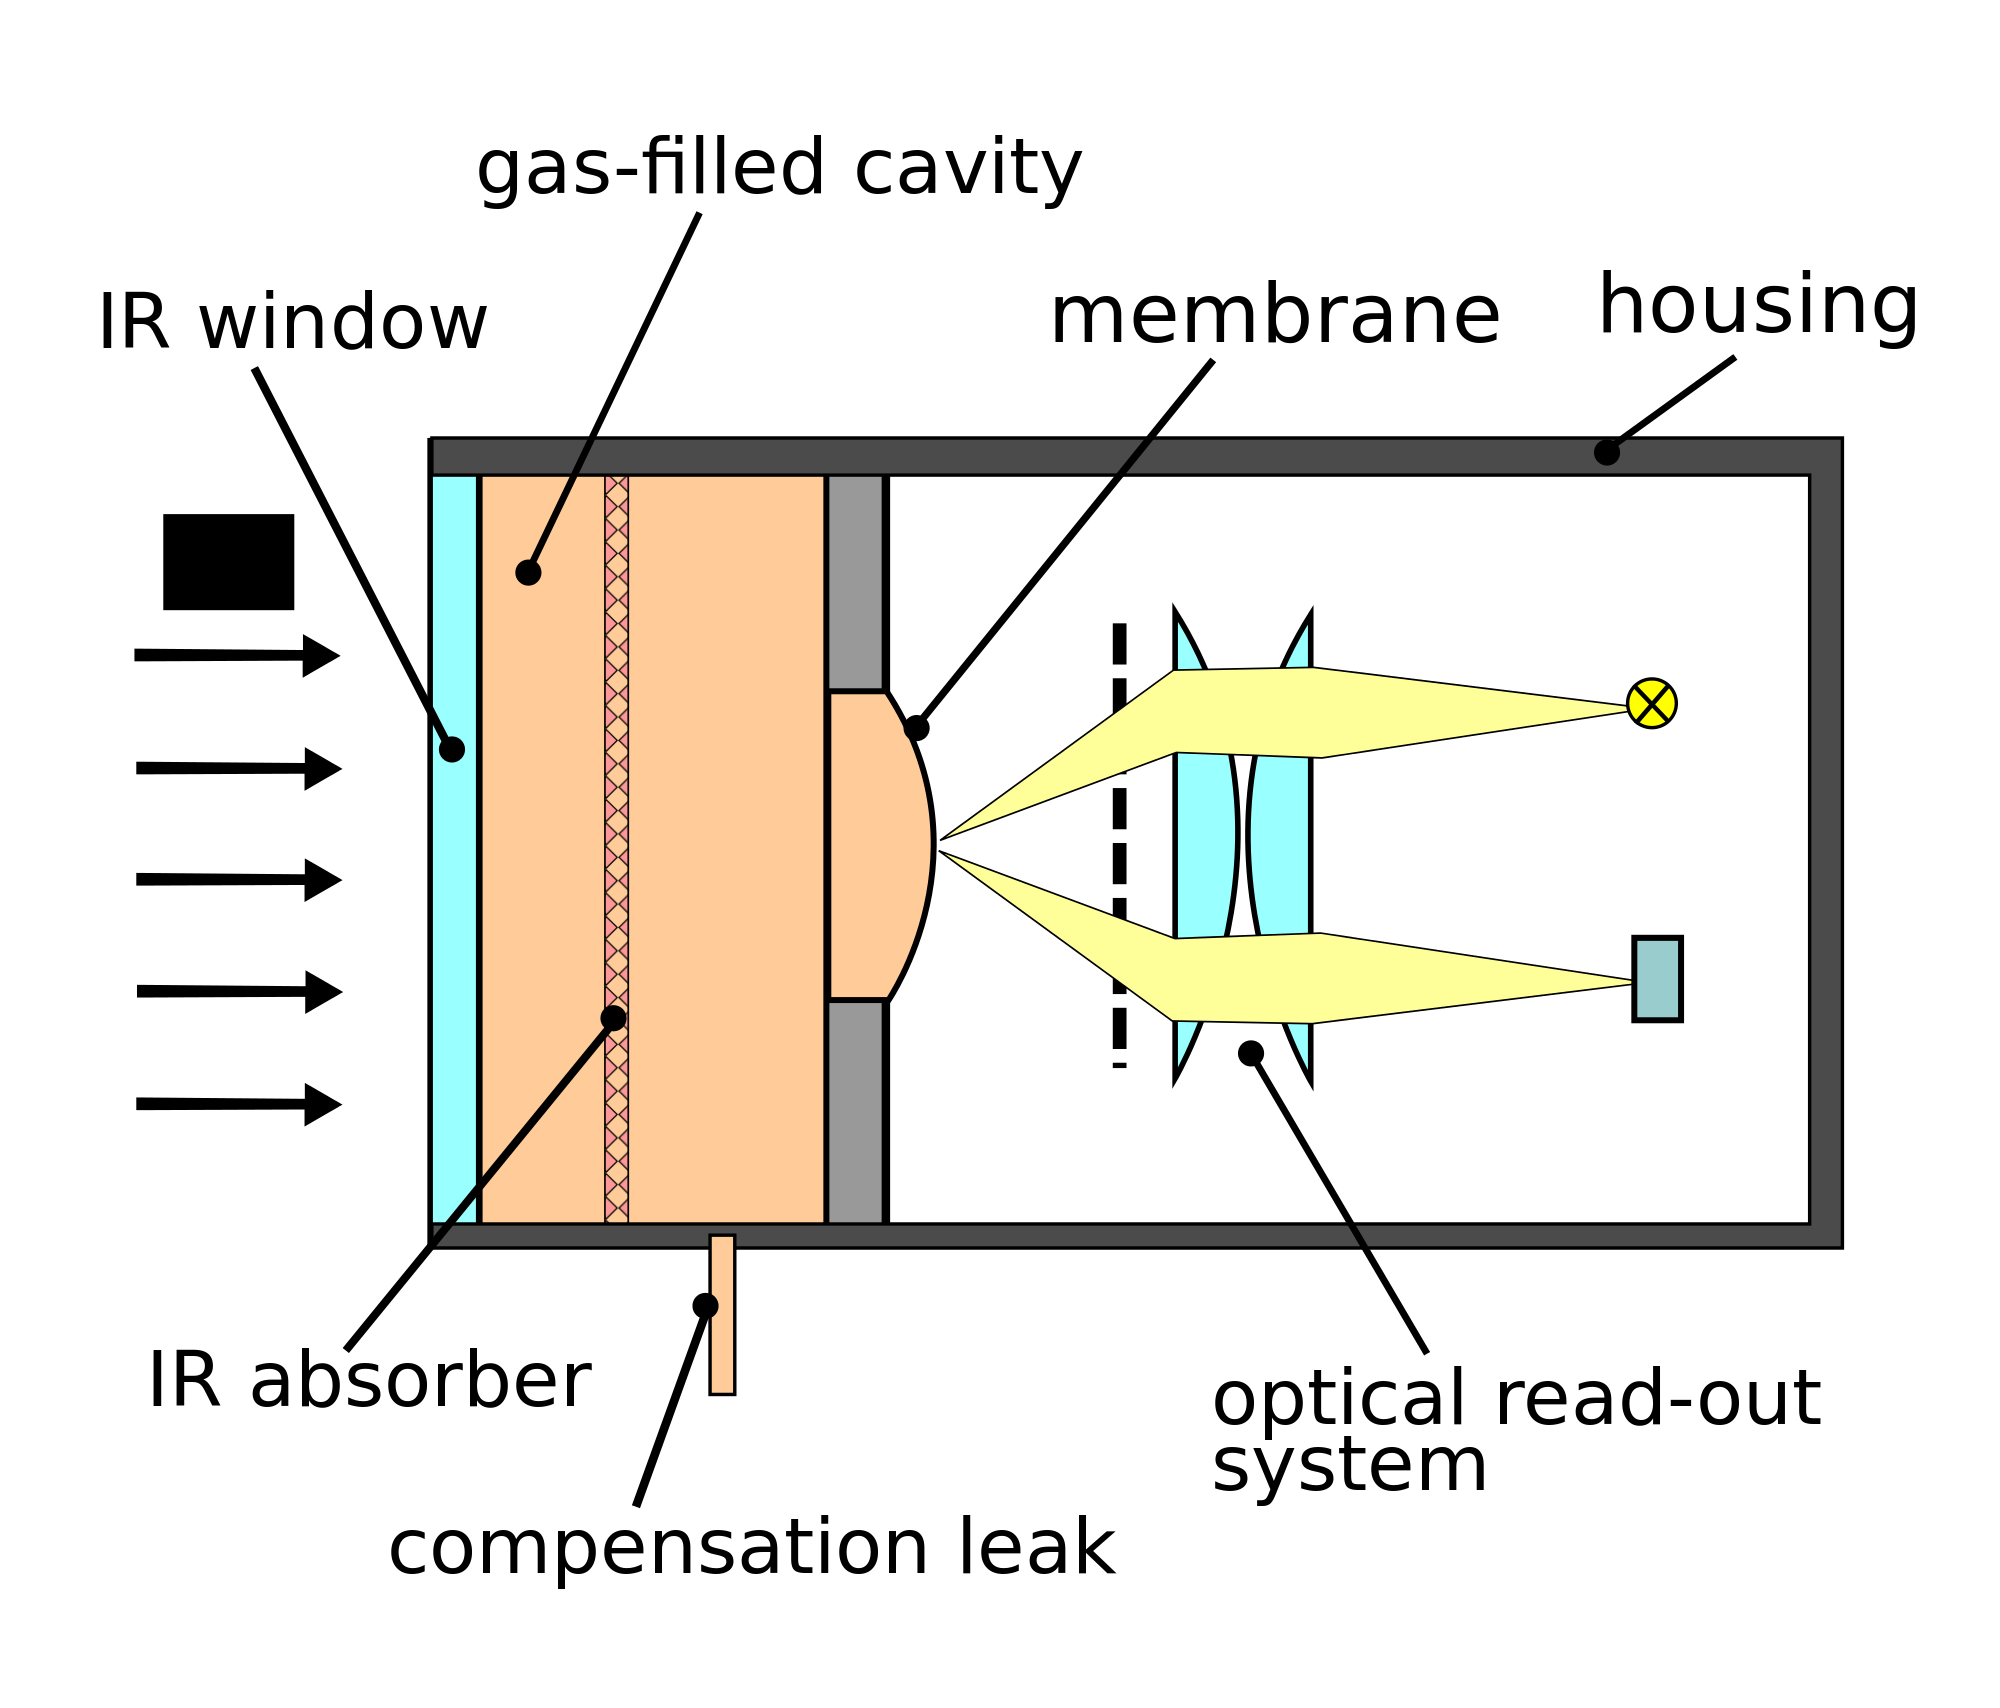
\includegraphics[width=9cm]{2000px-Golay_Cell_Schematic.png}
\end{frame}

\begin{frame}
\frametitle{Pneumatic detector model}

\end{frame}

\section{Back to insects}
\begin{frame}
\frametitle{Modelling the mechanoreceptor}
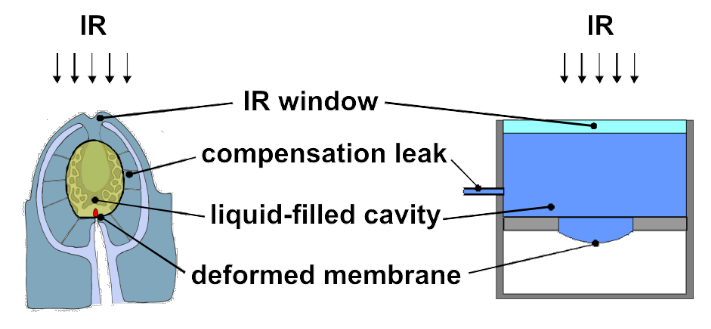
\includegraphics[width=10cm]{themodel.png}
\end{frame}

\begin{frame}
\frametitle{A bit of math}
\end{frame}

\begin{frame}
\frametitle{What is the best medium?}

\end{frame}

\section{A working prototype}
\begin{frame}
\frametitle{A built prototype}
From the Center of advanced european studies and research:\\
~\\
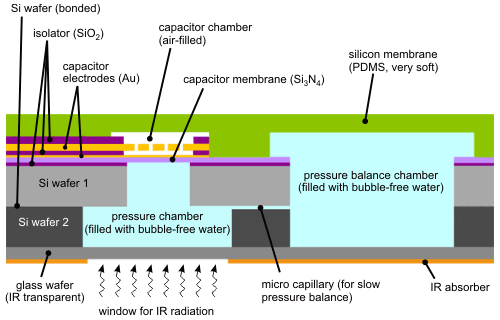
\includegraphics[width=8cm]{IR_sensor_abb_4_02.png}
\end{frame}
\begin{frame}
\frametitle{A built prototype}
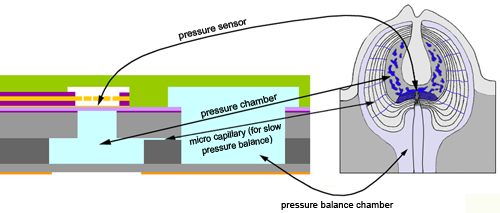
\includegraphics[width=10cm]{IR_sensor_abb_5_02.png}
\end{frame}

\section{Other detector for FIR}
\begin{frame}
\frametitle{Comparing Golay cells and pyroelectric detectors}

\end{frame}

\section{Conclusion}
\begin{frame}
\frametitle{Conclusion}

\end{frame}


%{
%\usebackgroundtemplate{\includegraphics[width=\paperwidth]{cyborg.jpg}}
%\setbeamertemplate{headline}{\includegraphics[width=\paperwidth]{cyborg.jpg}}
%\begin{frame}
%\vspace{6.cm}Thanks to Samuele, Romain, Tobias, \\Antoine, for useful input. More discussions \\will be needed!
%\end{frame}
%}

\end{document}
